%%Når du starter på en opgave skriver du \begin{opgave}{navnet på opgaven}{sværhedsgrad}, hvor sværhedsgraden skrives som 1,2 eller 3, hvor 3 er den sværeste. 
%%Når opgaven er slut skrives \end{opgave}. 
%%Såfremt der er delopgaver skrives delopgaver som \opg 
%
%%Eksempel på opgave 
%%\begin{opgave}{Polære koordinater}{1}
%  %Den kinetiske energi af et legeme, der bevæger sig i 2D-planet er
%  %i kartesiske koordinater ($x$ og $y$) givet ved ligning
%  %(1.11).
%  %
%  %\opg Beregn $\dt{x}$ og $\dt{y}$ i polære koordinater og vis
%  %derefter, at den kinetiske energi udtrykt i polære koordinater er
%  %givet ved ligning (1.12).
%%\end{opgave}
\chapter{Elektromagnetiske Bølger Opgaver}
\section*{træningsmatematik}

\begin{opgave}{Gradient}{1}
Find gradienten ($\v \nabla f$) af følgende funktioner:
\opg$f(x,y) = x$
\opg$f(x,y) = x^2-y^2$
\opg$f(x,y) = xy+\cos(xy)$
\opg$f(x,y,z) = x^3+xy^2+xyz$
\opg$f(x,y,z) = \frac{\cos(x)+\sin(y)}{z}$
\end{opgave}

\begin{opgave}{Divergens}{1}
Find divergensen ($\v \nabla \cdot \v F$) af følgende funktioner:
\opg$\v F(x,y) = x^2\xhat+y^2\yhat$
\opg$\v F(x,y) = \xy{x^2y}{-xy^2}$
\opg$\v F(x,y,z) = \sin(x)\xhat+\cos(y)\yhat$
\opg$\v F(x,y,z) = x^2\xhat+y^2\yhat-\mathrm{e}^z$
\opg$\v F(x,y) = \xyz{x^2\cos(y)}{y^2\cos(z)}{z^2\cos(x)}$
\opg$\v F(x,y) = \mathrm{e}^z(y^2\xhat+x^2\yhat)$
\end{opgave}

\begin{opgave}{Rotation}{2}
Find rotationen ($\v \nabla \times \v F$) af følgende funktioner:
\opg$\v F(x,y,z) = x^2\xhat+y^2\yhat$
\opg$\v F(x,y,z) = \xyz{x^2y}{-xy^2}{0}$
\opg$\v F(x,y,z) = \sin(x)\xhat+\cos(y)\yhat$
\opg$\v F(x,y,z) = -y^2\xhat+x^2\yhat-\mathrm{e}^z$
\opg$\v F(x,y,z) = \xyz{x^2\cos(y)}{y^2\cos(z)}{z^2\cos(x)}$
\opg$\v F(x,y,z) = \mathrm{e}^z(y^2\xhat+x^2\yhat)$
\end{opgave}



\begin{opgave}{Bølgeligningen}{2}
Er de følgende funktioner løsninger til bølgeligningen: 
$$
\frac{\partial^3 f}{\partial z^3} = \frac{1}{v^2}\frac{\partial^2 f}{\partial t^2}
$$
\opg $f(z,t) = z^2+t^2$
\opg $g(z,t) = \cos(kz-\omega t)+\sin(2kz+2\omega t)$
\opg $h(z,t) = \cos(kz)\cos(\omega t)$
\opg $i(z,t) = \cos(zt)$
\end{opgave}

\begin{opgave}{Gange matrix med vektor}{1}
Givet matricen $\v A$ og en vektor $\v v$, hvad er $\v A\v v$ for forskellige $\v v$
$$
\v A = \begin{bmatrix}
1&2\\0&3
\end{bmatrix}
$$
\opg $\v v = \xy{1}{0}$
\opg $\v v = \xy{0}{1}$
\opg $\v v = \xy{1}{1}$
\opg $\v v = \xy{1}{-1}$
\opg $\v v = \xy{3}{4}$
\opg Er der noget særligt ved nogle af vektorerne?
\end{opgave}

\begin{opgave}{Matrix multiplikation}{1}
Udregn følgende matrix regnestykker.
\opg $\begin{bmatrix}
1&0\\0&-1
\end{bmatrix}
\begin{bmatrix}
-5&2\\4&3
\end{bmatrix}
$
\opg $\begin{bmatrix}
1&2\\0&3
\end{bmatrix}
\begin{bmatrix}
1&2\\0&3
\end{bmatrix}
$
\opg $\begin{bmatrix}
1&2\\0&3
\end{bmatrix}
\begin{bmatrix}
3&-2\\0&1
\end{bmatrix}
$
\opg $\begin{bmatrix}
0&-1\\1&0
\end{bmatrix}^4
$
\opg $\begin{bmatrix}
0&0\\1&0
\end{bmatrix}^2
$
\opg $\begin{bmatrix}
1&2\\0&3
\end{bmatrix}
\begin{bmatrix}
7&-4\\1&-5
\end{bmatrix}
$
\end{opgave}

\begin{opgave}{Genereliserede vektorer (Bonus)}{2}
Vi har indtil vidre brugt vektorer til at beskrive størrelser der har en retning og en længde. Dette er en vigtig egenskab ved vektorer, men matematisk er alt der lægges sammen og ganges med skalarer som vektorer også vektorer. Blandt andet gælder det for polynomier (og alle andre funktioner). Det er derfor muligt at oversætte polynomier til koordinatvektorer. Vi vil her se på andengradspolynomier oversat til 3-diminsionelle vektorer.
\begin{equation}
\xyz{1}{0}{0} \equiv p_2(x)=x^2~~~~~\xyz{0}{1}{0} \equiv p_1(x) = x ~~~~\xyz{0}{0}{1} \equiv  p_0(x)=1
\end{equation}
\opg Hvad bliver parabelen $f(x) = ax^2+bx+c$ som koordinatvektor.
\opg Differentier $p_2$, $p_1$ og $p_0$, og brug det til at opstille matricen $\v D$ der beskriver differentiering.
\opg Find dobbelt differentialet $D^2$ og tripelt differenitalet $D^3$ med matrix multiplikation. Stemmer det overens med hvad du ville forvente?
\\\\Spejer man grafen i $y$-aksen svarer det til at skifte fortegn på inputtet af funktionen: $f(x)$ bliver $f(-x)$. Dette kaldes også for paritet.
\opg Find den matrix $\v P$ der beskriver paritets transformationen af en parabel.
\opg Find $\v D\v P$ og $\v P \v D$. Har det en betydning om man tager paritet før man differentierer eller efter.
\\\\
\emph{Bemærk}: Man ganger 3-dimensionelle matricer sammen på samme måde som 2-dimensionelle.
\begin{align}
\begin{bmatrix}
a&b&c\\
d&e&f\\
g&h&i
\end{bmatrix}
\xyz{v_1}{v_2}{v_3} &= \xyz{av_1+bv_2+cv_3}{dv_1+ev_2+fv_3}{gv_1+hv_2+iv_3}\\
\begin{bmatrix}
a_1&b_1&c_1\\
d_1&e_1&f_1\\
g_1&h_1&i_1
\end{bmatrix}
\begin{bmatrix}
a_2&b_2&c_2\\
d_2&e_2&f_2\\
g_2&h_2&i_2
\end{bmatrix}
&=\begin{bmatrix}
a_1a_2+b_1d_2+c_1g_2&a_1b_2+b_1e_2+c_1h_2&a_1c_2+b_1f_2+c_1i_2\\
d_1a_2+e_1d_2+f_1g_2&d_1b_2+e_1e_2+f_1h_2&d_1c_2+e_1f_2+f_1i_2\\
g_1a_2+h_1d_2+i_1g_2&g_1b_2+h_1e_2+i_1h_2&g_1c_2+h_1f_2+i_1i_2
\end{bmatrix}
\end{align}
\end{opgave}

\begin{opgave}{En elektrisk ladet plade}{1}
\label{em:gauss}
En elektrisk ladet plade med tykkelse $l$ ligger i $xy$-planen. Det elektriske felt er $E_z=A$ ovenover pladen, $E_z=Bz$ inde i pladen og $E_z=C$ under pladen.
$$
E_z = 
\begin{cases}
A~~\text{for}~~z\geq \frac{l}{2}\\
Bz~~\text{for}~~\frac{l}{2}\geq z\geq \frac{-l}{2}\\
C~~\text{for}~~\frac{-l}{2}\geq z
\end{cases}
$$
\opg Hvis den elektriske feltstyrke skal være kontinuert, Hvad er $A$ og $C$ udtryk i $B$
\opg Brug Gauss lov til at finde ladningstætheden langs $z$-aksen i de tre intervaller.
\end{opgave}

\begin{opgave}{Tre dimmensionelle ladningsfordelinger}{2}
Brug Gauss lov til at finde ladningsfordelingerne der giver de følgende felter:
\opg $\v{E} =A\hat{\v z}$
\opg $\v{E} =\frac{A}{3}(\hat{\v x}+\hat{\v y}+\hat{\v z})$
\opg $\v{E} =Az^2\hat{\v z}$
\opg $\v{E} =Ay^3\hat{\v y}$
\opg $\v{E} =A(z^2\hat{\v z}+y^3\hat{\v y})$
\opg $\v{E} =\frac{A}{xy}(\hat{\v x}+\hat{\v y}+\hat{\v z})$
\end{opgave}

\begin{opgave}{Integralformen af Gauss lov}{3}
Vi ser på samme plade som i opgave \ref{em:gauss}.
Flux er et mål for hvor meget et f.eks. elektrisk felt der går igennem en overflade: $$\Phi_E = \iint \v{E}\cdot\mathrm{d}\v{a} = \iint E \cos \theta \mathrm{d}a$$ $\theta$ er vinkelen imellem feltet og overfladens normalvektor. Gauss lov kan også skrives med integraler:
\begin{equation}
\oiint \v{E}\cdot \mathrm{d}\v{a} = \frac{Q_\text{enc}}{\varepsilon_0}
\end{equation}
Det betyder at fluxen ud igennem en lukket (p.g.a. cirkelen i integraltegnet) overflade er proportional med ladningen inden for overfladen.
\opg Find fluxen igennem et kvadrat med sidelængde $s$ inde i pladen der er parallelt med den.
\opg Find Find fluxen igennem et kvadrat med sidelængde $s$ inde i pladen der er vinkelret på den.
\opg Find fluxen ud igennem en kube med sidelængde $s$, som summen af fluxen igennem kuben sider.
\opg Burg integral formen af Gauss lov til at finde den gennemsnitlige ladningstæthed i kuben.
\\\\
~~(Hint: Integralet af en konstant er konstanten gange det område der er blevet integreret over, for dobbelte integraler er det et areal.)
\end{opgave}

\begin{opgave}{Faradays lov}{2}
Et varierende magnetisk felt skaber et elektrisk felt $\v E =Ay\omega\cos (\omega t)\hat{\v z}$.
\opg Brug Faradays lov til at finde $\frac{\partial \v B}{\partial t}$.
\opg Hvad er $\v B$.
\\\\~~(Hint: $\int \cos(ax)\mathrm{d}x=\frac{\sin(ax)}{a}+k$)
\end{opgave}

\begin{opgave}{Frekvens og bølgelængde}{1}
Find frekvensen af den elektromagnetiske stråling for de forskellige bølgelængder:
\opg Mikrobølger: $\lambda = 12,2\text{ cm}$
\opg Rødt lys: $\lambda = 632\text{ nm}$
\opg Röntgenstråling: $\lambda = 1,54\text{ Å}=0,154\text{ nm}$
\opg $\gamma$-stråling: $\lambda = 1,87\text{ pm}$
\end{opgave}

\begin{opgave}{Lineært Polariseret Lys}{1}
Lav en skitse af en opstilling der består af en horisontal polarisator og vertikal polarisator. Vi sender nu upolariseret lys ind i opstillingen. 
\opg Ser du noget lys efter den horisontale polarisator? Hvorfor? Hvorfor ikke?
\opg Hvorfor ser du ikke noget lys efter den vertikale polarisator? 
\opg Hvilken lineær polarisator skal du så sætte ind for at kunne se lys efter den vertikale polarisator? Hvor skal den placeres? 
\end{opgave}

\begin{opgave}{Forskellige måder at regne med Jones Matricer}{1}
I denne opgave skal I se, hvordan man kan finde den resulterende Jones vektor for polariseret lys, der sendes igennem et lineært polariseringsfilter med horisontal TA efterfulgt af en rotator, på to forskellige måder. I skal også se, at rækkefølgen er vigtig, når man regner med Jones matricer.  
\opg Tag den generelle Jones vektor for polariseret lys og gang denne med Jones matricen for filteret. Tag herefter den resulterende vektor og gang denne med Jones matricen for en rotator.
\opg Tag de to Jones matricer fra 1), gang dem sammen (husk rigtig rækkefølge) og gang så den resulterende matrix på den generelle Jones vektor. Sammenlign resultatet med det du fik i 1). Stemmer det med hvad du forventede? Hvorfor? Hvorfor ikke?
\opg Gentag 2) men prøv denne gang at bytte rundt på rækkefølgen af Jones matricerne. Sammenlign med resultatet fra 1) og 2). Stemmer det med hvad du forventede? Hvorfor? Hvorfor ikke?    
\end{opgave}

\begin{opgave}{Lineære Polarisatorer}{3}
I denne opgave skal vi kigge på transmission af lineært polariseret lys efter det har rejst gennem lineære polarisatorer. 
Først introduceres intensiteten af lyset som afhænger af det elektriske felt, $E$. 
\begin{equation}
I = \frac{1}{2}\varepsilon_0c\v{E}\v{E^*}, 
\end{equation}
hvor $\v{E^*}$ er den \emph{kompleks konjugerede} matrix af $\v{E}$. Man kompleks konjugerer en matrix ved at transponere den og skifte fortegn i de komplekse indgange (indgange, der indeholder $i$). I tilfælde, hvor matricen ikke er kompleks, transponerer man blot matricen. 
Hvis $\v{E} = \xy{a}{b}$ (som ikke er kompleks!), er
\begin{equation}
\v{E^*}=\begin{bmatrix} a & b \\ \end{bmatrix}.
\end{equation}
Derudover er $\v{E}^*\v{E} = |\v E_t|^2$. 
Transmissionen er forholdet mellem hvor meget intensitet, der kommer ud og hvor meget, der kommer ind, altså 
\begin{equation}
T = \frac{I_{\text{t}}}{I_{\text{i}}} = \frac{\v{E_{\text{t}}}\v{E_{\text{t}}^*}}{\v{E_{\text{i}}}\v{E_{\text{i}}^*}},
\end{equation}
hvor subcript t er for \emph{transmitteret} intensitet/elektrisk felt og subscript i er for \emph{indkommende} intensitet/elektrisk felt. For lineært polariseret lys er det indkommende elektriske felt, som tidligere nævnt, givet ved 
\begin{equation}
\v{E_{\text{i}}}=\xy{\cos\alpha}{\sin\alpha},
\end{equation}
hvor $\alpha$ er vinklen i forhold til polariseringsaksen. 
\opg Linært polariseret lys rejser gennem en lineær polarisator med horisontal TA. Beregn transmissionen som funktion af $\alpha$, $T(\alpha)$. 
\opg Skitsér $T(\alpha)$. Hvad fortæller den?\\

Der bruges nu tre lineære polarisatorer. En med vertikal TA, en med horisontal TA og en med en 45$\degree$ TA. Det oplyses at $\cos(45\degree) = \sin(45\degree) = \frac{1}{\sqrt{2}}$. 
\opg Beregn Jones Matricen for den lineære polarisator med en 45$\degree$ TA.  
\opg Beregn $T(\alpha)$ når lineært polariset lys rejser gennem Horisontal polarisator $\rightarrow$ 45$\degree$ polarisator $\rightarrow$ vertikal polarisator. 
\end{opgave}

\begin{opgave}{Faseforskydere}{3}
Et andet optisk element er en såkaldt \emph{faseforskyder}. Halvbølge plader og kvartbølge plader er eksempler på faseforskydere. Som navnet antyder påvirker en faseforskyder fasen i det elektriske felt. 

Det elektriske felt $E = E_0\cos(kz-\omega t)$ starter i (0,0), men det kan ændres ved at tilføje en fase, $\phi$. Fasen forskyder således startpunktet for bølgen, som det elektriske felt kan beskrives ved. Med fasen er $E = E_0\cos(kz-\omega t + \phi)$. Afstanden mellem to toppe i en cosinus funktion svarer til $2\pi$ i radianer, og man angiver derfor altid fasen som et tal gange $\pi$. Det elektrisk felt er her skrevet på sin reelle form, men i mange fysiske sammenhænge er det nemmere at skrive feltet på sin komplekse form. Den komplekse funktion $e^{iA} = \cos(A) + i\sin(A)$, hvor det første led er den real--delen og det sidste led er imaginær--delen. 
I arbejde med elektriske felter er blot et redskab, så den imaginære del af det elektriske felt har ingen fysisk betydning. Feltets komplekse form er givet ved 
\begin{equation}
E = E_0e^{i(kz - \omega t + \phi)}, 
\end{equation}
og da det elektriske felt består af en $x$-- og $y$--komponent er 
\begin{equation}
\v{E} = E_{0x}e^{i(kz - \omega t + \phi_x)}\hatvec{x} + E_{0y}e^{i(kz - \omega t + \phi_y)}\hatvec{y} = \left[E_{0x}e^{i\phi_x}\hatvec{x} + E_{0y}e^{i\phi_y}\hatvec{y}\right]e^{i(kz-\omega t)}. 
\end{equation}
En faseforskyder transformerer så
\begin{equation}
E_{0x}e^{i\phi_x} \,\,\,\,\, \text{til} \,\,\,\,\, E_{0x}e^{i(\phi_x + \varepsilon_x)}
\end{equation}
og 
\begin{equation}
E_{0y}e^{i\phi_y} \,\,\,\,\, \text{til} \,\,\,\,\, E_{0y}e^{i(\phi_y + \varepsilon_y)},
\end{equation}
hvor $\varepsilon_x$ og $\varepsilon_y$ kaldes for \emph{slow axis} og \emph{fast axis}, og de er altså en ekstra fase. 
Jones Matricen for en faseforskyder er derfor 
\begin{equation}
\v{M} = \begin{bmatrix}
e^{i\varepsilon_x} & 0 \\
0 & e^{i\varepsilon_y} \\
\end{bmatrix}.
\end{equation}
En faseforskyder kan f.eks. være enten en halvbølge plade eller kvartbølge plade. Differencen mellem $\varepsilon_x$ og $\varepsilon_y$ er det, der afgør, om det er den ene eller anden. Hvis $|\varepsilon_x-\varepsilon_y| = \pi$ er den en halvbølgeplade, mens den er en kvartbølge plade når $|\varepsilon_x-\varepsilon_y| = \frac{\pi}{2}$. 

Vi skal nu se på en opstilling, der i rækkefølge består af en kvartbølgeplade og en lineær polaristor med vertikal TA. Lyset er til at starte med horisontalt lineært polariseret. 

Vi ønsker at kunne rotere kvartbølge pladen med en vinkel $\theta$ og dermed bestemme transmissionen af lyset som funktion af denne vinkel. Jones Matricen for kvartbølgepladen $M$ er derfor ikke nok, da den ikke tager højde for, at kvartbølgepladen og skal rotere. Jones Matricen for en roterende kvartbølge plade er derfor 
\begin{equation}
\tilde{\v{M}} = \v{R} \v{M} \v{R}^{-1}, 
\end{equation}
hvor $\v{R}$ er rotator matricen og 
\begin{equation}
\v{R}^{-1} = \begin{bmatrix}
\cos\theta & \sin\theta \\
-\sin\theta & \cos\theta \\
\end{bmatrix}.
\end{equation}
\opg Beregn $\tilde{\v{M}}$ for en kvartbølgeplade. 
\opg Beregn $T_v(\theta)$ for når lyset er rejst gennem opstillingen. \emph{Hint: $i^2=-1$}. Skitsér $T_v(\theta)$. 
\opg Beregn $T_h(\theta)$ for samme opstilling, men hvor den vertikale lineær polarisator nu er skiftet ud med en horisontal lineær polarisator. Skitser $T_h(\theta)$
\opg Beregn $\tilde{\v{M}}$ for en halvbølge plade og gentag beregning er $T_{v/h}(\theta)$ for opstillingen når den indeholder en vertikal lineære polarisator og når den indeholder en horisontal lineær polarisator. Skitsér $T_v(\theta)$ og $T_h(\theta)$. 
\end{opgave}

\newpage
\chapter{Elektromagnetiske bølger Facitliste}
\begin{opgave}{Gradient}{1}
\opg $f(x,y) = x ~~~~\v\nabla f(x,y) = \xhat = \xy{1}{0}$
\opg $f(x,y) = x^2-y^2 ~~~~\v\nabla f(x,y) = x\xhat-y\yhat=\xy{x}{y}$
\opg $f(x,y) = xy+\cos(xy) ~~~~\v\nabla f(x,y) = (y-x\sin(xy))\xhat+(x-y\sin(xy))\yhat = \xy{y-x\sin(xy)}{x-y\sin(xy}$
\opg $f(x,y,z) = x^3+xy^2+xyz ~~~~\v\nabla f(x,y) = (3x^2+y^2+yx)\xhat+(2xy+xz)\yhat+xy\zhat = \xyz{3x^2+y^2+yz}{2xy+xz}{xy}$
\opg $f(x,y,z) = x ~~~~\v\nabla f(x,y) = \frac{-\sin(x)}{z}\xhat+\frac{\cos(y)}{z}\yhat-\frac{1}{z^2}\zhat = \frac{1}{z}\xyz{-\cos(x)}{\sin(y)}{-1/z}$
\end{opgave}


\begin{opgave}{Divergens}{1}
Find divergensen ($\v \nabla \cdot \v F$) af følgende funktioner:
\opg$\v F(x,y) = x^2\xhat+y^2\yhat~~~~\v\nabla\cdot F = 2x+2y$
\opg$\v F(x,y) = \xy{x^2y}{-xy^2}~~~~\v\nabla\cdot F = 2xy-2xy= 0$
\opg$\v F(x,y,z) = \sin(x)\xhat+\cos(y)\yhat~~~~\v\nabla \cdot F = \cos(x)-\sin(y)$
\opg$\v F(x,y,z) = x^2\xhat+y^2\yhat-\mathrm{e}^z~~~~\v\nabla\cdot F = 2x+2y+\mathrm{e}^z$
\opg$\v F(x,y) = \xyz{x^2\cos(y)}{y^2\cos(z)}{z^2\cos(x)}~~~~\v\nabla\cdot F = 2x\cos(y)+2y\cos(z)+2z\cos(x)$
\opg$\v F(x,y) = \mathrm{e}^z(y^2\xhat+x^2\yhat)~~~~\v\nabla\cdot F = 0$
\end{opgave}

\begin{opgave}{Rotation}{2}
Find rotationen ($\v \nabla \times \v F$) af følgende funktioner:
\opg$\v F(x,y,z) = x^2\xhat+y^2\yhat ~~~~\v\nabla \times F = \v 0$
\opg$\v F(x,y,z) = \xyz{x^2y}{-xy^2}{0} ~~~~\v\nabla \times F =\xyz{0}{0}{-x^2-y^2}$
\opg$\v F(x,y,z) = \sin(x)\xhat+\cos(y)\yhat ~~~~\v\nabla \times F =\v 0$
\opg$\v F(x,y,z) = -y^2\xhat+x^2\yhat-\mathrm{e}^z ~~~~\v\nabla \times F =2x+2y$
\opg$\v F(x,y,z) = \xyz{x^2\cos(y)}{y^2\cos(z)}{z^2\cos(x)} ~~~~\v\nabla \times F =xyz{y^2\sin(z)}{-z^2\sin(x)}{-x^2\sin(y)}$
\opg$\v F(x,y,z) = \mathrm{e}^z(y^2\xhat+x^2\yhat) ~~~~\v\nabla \times F =\xyz{-\mathrm{e}^zx^2}{-\mathrm{e}^zy^2}{2\mathrm{e}^z(x-y)}$
\end{opgave}


\begin{opgave}{Bølgeligningen}{2}
Er de følgende funktioner løsninger til bølgeligningen: 
$$
\frac{\partial^2f}{\partial z^2} = \frac{1}{v^2}\frac{\partial^2 f}{\partial t^2}
$$
Man differentierer funktionen dobbelt til både $t$ og $z$. Er der kun en faktor til forskel er det en løsning.
\opg 
\begin{align*}
f(z,t) &= z^3+t^3\\
\frac{\partial f}{\partial z} &= 3z^2\\
\frac{\partial^2 f}{\partial z^2} &== 6z\\
\frac{\partial f}{\partial t} = 3t\\
\frac{\partial^2 f}{\partial t^2} = 6t
\end{align*}
Det er ikke en løsning.
\opg Her bruges kædereglen til differentiere funktionerne.
\begin{align*}
g(z,t) &=\cos(kz-\omega t)+\sin(2kz+2\omega t)\\
\frac{\partial g}{\partial z} &= -k\cos(kz-\omega t)+2k\cos(2kz-2\omega t)\\
\frac{\partial^2 g}{\partial t^2} &=-k^2\sin(kz-\omega t)-4k^2\sin(2kz-2\omega t)\\
\frac{\partial g}{\partial t} &= \omega\sin(kz-\omega t) -2\omega \cos(2kz-2\omega t)\\
\frac{\partial^2 g}{\partial t^2} &= -\omega^2\cos(kz-\omega t) - 4\omega^2\cos(2kz-2\omega t)\\
-k^2\frac{\partial^2 g}{\partial z^2} &= -\omega^2 \frac{\partial^2 g}{\partial t^2}~~\text{Gælder, så det er en løsning.}\\
v&=\frac{\omega}{k}~~\text{~Er bølgens hastighed.} 
\end{align*}
Bølgeligningen hører til en kategori af velopdragne differentialligninger hvor summen af to løsninger også er en løsning. De kaldes lineære differentialligninger.
\opg
\begin{align*}
h(z,t) &= \cos(kz)\cos(\omega t)\\
\frac{\partial h}{\partial z} &= -k\sin(kz)\cos(\omega t)\\
\frac{\partial^2 h}{\partial z^2} &= -k^2\cos(kz)\cos(\omega t)\\
\frac{\partial h}{\partial t} &= -\omega \cos(kz)\sin(\omega t)\\
\frac{\partial^2 h}{\partial t^2} &= -\omega^2 \cos(kz)\cos(\omega t)\\
-k^2\frac{\partial^2 h}{\partial z^2} &= -\omega^2\frac{\partial^2 h}{\partial t^2}~~\text{Det er en løsning}\\
v &= \frac{\omega}{k}~~\text{er hastigheden af bølgen}
\end{align*}
Dette er iøvrigt en stående bølge. Den kan også meskrives som to bølger med den halve amplitude og rejsende i hver sin retning.
\opg
\begin{align*}
i(z,t) &= \cos(zt)\\
\frac{\partial i}{\partial z} &= -t\sin(zt)\\
\frac{\partial^2 i}{\partial^2 z} &= -t^2\cos(zt)\\
\frac{\partial i}{\partial t} &= -z\sin(zt)\\
\frac{\partial^2 i}{\partial t^2} &= -z^2\cos(zt)
\end{align*}
Det er ikke en løsning.
\end{opgave}

\begin{opgave}{Gange matrix med vektor}{1}
Givet matricen $\v A$ og en vektor $\v v$, hvad er $\v A\v v$ for forskellige $\v v$
$$
\v A = \begin{bmatrix}
1&2\\0&3
\end{bmatrix}
$$
\opg $\v v = \xy{1}{0}~~~~\v A\v v  = \xy{1}{0}$
\opg $\v v = \xy{0}{1}~~~~\v A\v v  = \xy{2}{3}$
\opg $\v v = \xy{1}{1}~~~~\v A\v v  = \xy{3}{3}$
\opg $\v v = \xy{1}{-1}~~~~\v A\v v  = \xy{-1}{-3}$
\opg $\v v = \xy{3}{4}~~~~\v A\v v  = \xy{11}{12}$
\opg Er der noget særligt ved nogle af vektorerne? $\xy{1}{0}$ og $\xy{1}{1}$ er egenvektorer for $\v A$. De giver sigselv gange en faktor.
\end{opgave}


\begin{opgave}{Matrix multiplikation}{1}
Udregn følgende matrix regnestykker.
\opg $\begin{bmatrix}
1&0\\0&-1
\end{bmatrix}
\begin{bmatrix}
-5&2\\4&3
\end{bmatrix} = \begin{bmatrix}
-5&2\\-4&-3
\end{bmatrix}
$
\opg $\begin{bmatrix}
1&2\\0&3
\end{bmatrix}
\begin{bmatrix}
1&2\\0&3
\end{bmatrix}=
\begin{bmatrix}
1&8\\0&9
\end{bmatrix}
$
\opg $\begin{bmatrix}
1&2\\0&3
\end{bmatrix}
\begin{bmatrix}
3&-2\\0&1
\end{bmatrix}=
\begin{bmatrix}
3&0\\0&3
\end{bmatrix}
$
\opg $\begin{bmatrix}
0&-1\\1&0
\end{bmatrix}^4=\begin{bmatrix}
1&0\\0&1
\end{bmatrix}
$
\opg $\begin{bmatrix}
0&0\\1&0
\end{bmatrix}^2
=
\begin{bmatrix}
0&0\\0&0
\end{bmatrix}
$
\opg $\begin{bmatrix}
1&2\\0&3
\end{bmatrix}
\begin{bmatrix}
7&-4\\1&-5
\end{bmatrix}
=
\begin{bmatrix}
9&-14\\
3&15
\end{bmatrix}
$
\end{opgave}

\begin{opgave}{Genereliserede vektorer}{2}
\opg $f(x) = ax^2+bx+c$ bliver $ap_2(x)+bp_1(x)+cp_0(x) = \xyz{a}{b}{c}$.
\opg $\frac{d}{dx}p_2(x) = 2x = 2p_1(x)$\\
$\frac{d}{dx}p_1(x) = 1 = p_0(x)$\\
$\frac{d}{dx}p_0(x) = 0$\\
De differentierede koordinatvektorer sættes ind som søjler i matricen.\\
$\v D = \begin{bmatrix}
0&0&0\\
2&0&0\\
0&1&0
\end{bmatrix}
$
\opg $\v D^2 = \begin{bmatrix}
0&0&0\\
0&0&0\\
2&0&0
\end{bmatrix}$\\
$\v D^3 = \begin{bmatrix}
0&0&0\\
0&0&0\\
0&0&0
\end{bmatrix}$
\opg
Samme fremgangsmåde som opgave 1\\
$p_2(-x) = (-x)^2 = x^2=p_2(x)$\\
$p_1(-x) = -x = -p_1(x)$\\
$p_0(-x) = 1 =p_1(x)$\\
$\v P = \begin{bmatrix}
1&0&0\\
0&-1&0\\
0&0&1
\end{bmatrix}$
\opg
$\v D \v P=\begin{bmatrix}
0&0&0\\
2&0&0\\
0&-1&0
\end{bmatrix}$\\
$\v P\v D = \begin{bmatrix}
0&0&0\\
-2&0&0\\
0&1&0
\end{bmatrix}$
\end{opgave}

\begin{opgave}{En elektrisk ladet plade}{1}
\opg Hvis feltet skal være kontinuert vil $E_z\left(\frac{l}{2}\right)=A=B\frac{l}{2}$ på oversiden og tilsvarende: $E_z\left(\frac{-l}{2}\right)=-B\frac{l}{2}=C$.
\opg $\rho = \v \nabla \v E \varepsilon_0 = \frac{\partial E_z}{\partial z}\varepsilon_0$. På begge sider af pladen er det nul. inde i pladen er det: $\rho = B\varepsilon_0$
\end{opgave}

\begin{opgave}{Tre dimmensionelle ladningsfordelinger}{2}
Brug Gauss lov til at finde ladningsfordelingerne der giver de følgende felter:
\opg $\v{E} =A\hat{\v z} = 0$
\opg $\v{E} =\frac{A}{3}(\hat{\v x}+\hat{\v y}+\hat{\v z}) = 0$
\opg $\v{E} =Az^2\zhat = 2Az$
\opg $\v{E} =Ay^3\yhat = 3Ay^2$
\opg $\v{E} =A(z^2\hat{\v z}+y^3\hat{\v y}) = A(2z+3y)$
\opg $\v{E} =\frac{A}{xy}(\hat{\v x}+\hat{\v y}+\hat{\v z}) = -A\left(\frac{1}{x^2y}+\frac{1}{xy^2}\right)$
\end{opgave}

\begin{opgave}{Integralformen af Gauss lov}{3}
\opg
Siden kvadratet er parallelt med pladen ligge hele kvadratet i samme $z$. $\v E$-feltet er vinkelret på pladen så, med hjælp fra hintet er fluxen:
$$
\Phi_E(z) = \iint E_z \mathrm{d}a = E_zs^2 = Bzs^2
$$
\opg
Er kvadratet vinkelret på pladen vil $\cos\theta=0$ derfor er fluxen det også.
\opg
Husk at man måler fluxen ud af kuben. Toppen og bunden af kuben er parallelle med pladen, så de bidrager med $Bzs^2$ resten af siderne er vinkelrette så de bidrager ikke.
Placeres kuben med centrum i en højde $z_0$ bliver den fluxen ud igennem den:
$$
\Phi_E = \Phi_E(z_0+\tfrac{l}{2})-\Phi_E(z_0-\tfrac{l}{2})=Bs^3
$$
Ud fra integralformen af Gauss lov findes den indesluttede ladning.
$$
Q_\text{encl} = Bs^3\varepsilon_0
$$
Derefter findes ladningstætheden ved at dele med rumfanget af kuben
$$
\rho_\text{gns} = \frac{Q_\text{encl}}{s^3} = B\varepsilon_0
$$
Dette virker kun fordi ladningstætheden er konstant, men gøres $s$ mindre vil man opnå et gradvist bedre resultat.
\end{opgave}

\begin{opgave}{Faradays lov}{2}
\opg Man tager rotationenaf $\v E$-feltet og bruger Faradays lov til at finde $\frac{\partial \v B}{\partial t}$.
$$
\frac{\partial \v B}{\partial t} = -\v \nabla \times \v E = -A\omega\cos(\omega t)\xhat
$$
\opg
Siden integration er det modsatte af diffentiation indsættes det i det givne integral.
$$
\v B = \int \frac{\partial \v B}{\partial t}\mathrm{d}t = -A\omega\xhat\int\cos(\omega t)\mathrm{d}t = -A\xhat\sin(\omega t)
$$
Der kan egentligt også være en konstant del af $\v E$-feltet, men vi kan ikke vide noget om den og antager derfor at den er nul.
\end{opgave}

\begin{opgave}{Frekven og bølgelængde}{1}
Brug sammenhængen $c = \nu\lambda\iff\nu=\frac{c}{\lambda}$.
\opg Mikrobølger: $\lambda = 12,2\text{ cm}~~~~~\nu = 2,46 \mathrm{GHz} = 2,46\cdot 10^9\mathrm{Hz}$
\opg Rødt lys: $\lambda = 632\text{ nm}~~~~~\nu = 474 \mathrm{THz} = 4,74\cdot 10^{12}\mathrm{Hz}$
\opg Röntgenstråling: $\lambda = 1,54\text{ Å}=0,154\text{ nm}~~~~~\nu = 1,95 \mathrm{EHz} = 2,46\cdot 10^{18}\mathrm{Hz}$
\opg $\gamma$-stråling: $\lambda = 1,87\text{ pm}~~~~~\nu = 160 \mathrm{EHz} = 2,46\cdot 10^{20}\mathrm{Hz}$
\end{opgave}

\begin{opgave}{Lineært Polariseret Lys}{1}
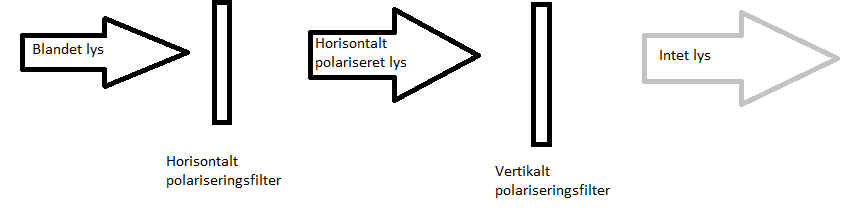
\includegraphics[width = \textwidth]{elektrodynamik/polskitse.png}
\opg Siden upolariseret lys består af en blanding af alle polariseringer vil noget af det komme igennem polariseringsfilteret.
\opg Efter det horisontale polariseringsfilter er lyset horisontalt polariseret, derfor kan intet komme igennem det vertikale polariseringsfilter.
\opg Indsættes et diagonalt polariseringsfilter imellem de to oprindelige filtre, vil det diagonale filter tillade noget af det horisontalt polariserede lys at passere, men bagefter er det være diagonalt polariseret, så noget af det kommer også igennem.
\end{opgave}

\begin{opgave}{Forskellige måder at regne med Jones Matricer}{1}
Generelt polariseret lys har Jones vektoren: $\v v = \xy{\cos \alpha}{\sin \alpha}$. Polariseringsfilteret har Jones matricen: 
$\v P = \begin{bmatrix}
1&0\\0&0
\end{bmatrix}$.
Rotatoren har Jones matricen: $\v R = \begin{bmatrix}
\cos\beta & -\sin\beta\\\sin\beta&\cos\beta
\end{bmatrix}$
\opg Filteret gange vektoren er:
$$
\begin{bmatrix}
1&0\\0&0
\end{bmatrix}
\xy{\cos\alpha}{\sin\alpha} = \xy{cos\alpha}{0}
$$
Denne vektor gange rotatoren bliver:
$$
\begin{bmatrix}
\cos \beta&-\sin\beta\\\sin \beta&\cos\beta
\end{bmatrix}
\xy{\cos\alpha}{0}=
\xy{\cos\alpha\cos\beta}{\cos\alpha\sin\beta}
$$
Hvis man vil kan man bruge trigonometriske identiteter til at omskrive det, men det bliver ikke pænere af det.
$$
\xy{\cos\alpha\cos\beta}{\cos\alpha\sin\beta}=
\frac{1}{2}\xy{\cos(\alpha-\beta)+\cos(\alpha+\beta)}{\sin(\alpha+\beta)-\sin(\alpha-\beta)}
$$
\opg Ganger man matricerne sammen får man:
$$
\v R\v P=
\begin{bmatrix}
\cos\beta&\sin\beta\\0&0
\end{bmatrix}
$$
Ganges denne matrix på vektoren fåes
$$
\begin{bmatrix}
\cos\beta & \sin\beta \\ 0 & 0
\end{bmatrix}
\xy{\cos\alpha}{\sin\alpha}=
\xy{\cos\alpha\cos\beta}{\cos\alpha\sin\beta}
$$
Rækkefølgen har ingen betydning. Dette gælder generelt for matricer og vektorer. Det kaldes den distributive lov.$\v A\v B\v C=(\v A\v B)\v C=\v A(\v B\v C)$
\opg
I den anden rækkefølge bliver det:
$$
\v P(\v R \v v ) = 
\begin{bmatrix}
1&0\\0&0
\end{bmatrix}
\begin{bmatrix}
\cos\beta & -\sin\beta\\\sin\beta&\cos\beta
\end{bmatrix}
\xy{\cos\alpha}{\sin\alpha}
=
\begin{bmatrix}
1&0\\0&0
\end{bmatrix}
\xy{\cos\alpha\cos\beta-\sin\alpha\sin\beta}{\cos\alpha\sin\beta+\sin\alpha\cos\beta}=
\xy{\cos\alpha\cos\beta-\sin\alpha\sin\beta}{0}
$$
Ganges matricerne samme først bliver det.
$$
\v P(\v R \v v ) = 
\begin{bmatrix}
1&0\\0&0
\end{bmatrix}
\begin{bmatrix}
\cos\beta & -\sin\beta\\\sin\beta&\cos\beta
\end{bmatrix}
\xy{\cos\alpha}{\sin\alpha}=
\begin{bmatrix}
\cos\beta&-\sin\beta\\
0&0
\end{bmatrix}
\xy{\cos\alpha}{\sin\beta}
=
\xy{\cos\alpha\cos\beta-\sin\alpha\sin\beta}{0}
$$
Bemærk at rækkefølgen af matricerne har betydning.
\end{opgave}

\begin{opgave}{Lineære Polarisatorer}{3}
\opg Den horisontale polarisator har Jones matricen $\v H=\begin{bmatrix}
1&0\\0&0
\end{bmatrix}$
Det transmiterede lys har Jones vektoren:
$$
\v E_t = \v H \v E_i = \begin{bmatrix}
1&0\\0&0
\end{bmatrix}
\xy{\cos\alpha}{\sin\alpha}
=
\xy{\cos\alpha}{0}
$$
Nu kan intensiteterne findes ud fra Jones vektorerne. Til $I_i$ anvendes Pythagoras sætning for en trekant i enhedscirkelen.
$$
|\v E_i|^2=\cos^2\alpha+\sin^2\alpha=1
$$
$$
|\v E_t|^2=\cos^2\alpha
$$
Transmitansen er dermed:
$$
T(\alpha)=\frac{|\v E_t|^2}{|\v E_i|^2}=\cos^2\alpha
$$
\opg Den blå graf på figuren er $T(\alpha)$
\opg Den generelle form for et lineært polariseringsfilter findes i kompendiet ligning (6.28). Den er:
$$
\v P(\theta)=\begin{bmatrix}
\cos^2\theta&\cos\theta\sin\theta\\
\cos\theta\sin\theta&\sin^2\theta
\end{bmatrix}
$$
Indsættes $\theta=45^\circ$ bliver alle indgangene $\frac{1}{2}$.
$$
\v P(45^\circ) = \begin{bmatrix}\tfrac{1}{2}&\tfrac{1}{2}\\\tfrac{1}{2}&\tfrac{1}{2}\end{bmatrix} = \frac{1}{2} \begin{bmatrix}
1 & 1 \\
1 & 1 \\
\end{bmatrix}
$$
%\opg
%Jones vektoren for lineært polariseret lys sendt igennem et diagonalt filter er:
%$$
%\v D\v E_i = \begin{bmatrix}
%\tfrac{1}{2}&\tfrac{1}{2}\\\tfrac{1}{2}&\tfrac{1}{2}
%\end{bmatrix}
%\xy{\cos\alpha}{\sin\alpha}
%=
%\frac{1}{2}\xy{\cos\alpha+\sin\alpha}{\cos\alpha+\sin\alpha}
%$$
%$|\v E_i|^2$ er uændret og lig 1, så $T=|\v E_t|^2$.
%$$
%T(\alpha)=\frac{1}{4}((\cos\alpha+\sin\alpha)^2+(\cos\alpha+\sin\alpha)^2)=\frac{1}{2}(\cos^2\alpha+\sin^2\alpha+2\cos\alpha\sin\alpha)
%=
%\frac{1}{2}+\cos\alpha\sin\alpha
%$$
%Denne funktion er plottet i rødt på figuren. Som man kan se er den forskudt $45^\circ$ i forhold til et horisontalt polariseringsfilter.
%Det er helt fint at slutte er, men det er muligt at gøre resultatr pænere med et par trigonometriske identiteter.
%$
%\cos u\sin v = \frac{1}{2}(\sin(u+v)-\sin(u-v))
%$
%Så bliver transmitansen:
%$$
%T(\alpha) = \frac{1}{2}+\frac{1}{2}(\sin(2\alpha)-\sin(0))=\frac{1}{2}(1+\sin(2\alpha))
%$$
%Herefter bruges:
%$
%\cos(u-90^\circ) = \sin u
%$
%
%$$
%T(\alpha) = \frac{1}{2}(1+\cos(2\alpha-90^\circ))=\frac{1}{2}(1+\cos(2(\alpha-45^\circ)))
%$$
%Den sidste identitet der bruges er: $\cos^2u=\frac{1}{2}(1+\cos(2u))$
%$$
%T(\alpha) = \cos^2(\alpha-45^\circ)
%$$
\includegraphics[scale=1]{elektrodynamik/Emskitse.eps}
\opg
Der er to måder at løse denne opgave på. Man kan enten gange de relevante Jones matricer på vektoren en af gangen, eller man kan gange matricerne sammen og derefter gange med vektoren. Her demonstreres kun den anden metode.
De relvante matricer er:
$$
\v H = \begin{bmatrix}
1&0\\0&0
\end{bmatrix}
~~~~~\v D=
\frac{1}{2}\begin{bmatrix}
1&1\\1&1
\end{bmatrix}
~~~~\v V = \begin{bmatrix}
0&0\\0&1
\end{bmatrix}
$$
Bemærk rækkefølgen af matricerne, da lyset først passerer den horisontale polarisator er den tilsvarende. Den endelige Jones matrix er dermed:
$$
\v M = \v{VDH}=
\frac{1}{2}
\begin{bmatrix}
0&0\\0&1
\end{bmatrix}
\begin{bmatrix}
1&1\\1&1
\end{bmatrix}
\begin{bmatrix}
1&0\\0&0
\end{bmatrix}
=
\frac{1}{2}
\begin{bmatrix}
0&0\\0&1
\end{bmatrix}
\begin{bmatrix}
1&0\\1&0
\end{bmatrix}
=
\frac{1}{2}
\begin{bmatrix}
0&0\\1&0
\end{bmatrix}
$$
Nu kan $\v E_t$ findes
$$
\v E_t = \v M \v E_i = \frac{1}{2}\begin{bmatrix}
0&0\\0&1
\end{bmatrix}
\xy{\cos\alpha}{\sin\alpha}
=
\frac{1}{2}\xy{0}{\cos\alpha}
$$
Så kan $T(\alpha)$ findes
$$
T(\alpha) = \frac{|\v E_t|^2}{|\v E_i|^2}=\frac{1}{4}\cos^2\alpha
$$
%Hvilket iøvrigt kan omskrives til:
%$$
%\frac{\cos^2(\alpha-90^\circ)}{4}
%$$
Intensiteten mindskes med en faktor 4 og det resulterende lys er vandret polariseret.
\end{opgave}

\begin{opgave}{Faseforskydere}{3}
\opg $\tilde{\v M}$ bliver
\begin{equation*}
\tilde{\v{M}} = 
\begin{bmatrix}
\cos\theta & -\sin\theta \\
\sin\theta & \cos\theta \\
\end{bmatrix}
\begin{bmatrix}
e^{i\varepsilon_x} & 0 \\
0 & e^{i\varepsilon_y} \\
\end{bmatrix}
\begin{bmatrix}
\cos\theta & \sin\theta \\
-\sin\theta & \cos\theta \\
\end{bmatrix}
=
\begin{bmatrix}
e^{i\varepsilon_x} \cos^2 \theta + e^{i\varepsilon_y} \sin^2 \theta & \left( e^{i\varepsilon_x}-e^{i\varepsilon_y} \right)\cos\theta\sin\theta \\
\left( e^{i\varepsilon_x}-e^{i\varepsilon_y} \right)\cos\theta\sin\theta & e^{i\varepsilon_x} \sin^2 \theta + e^{i\varepsilon_y} \cos^2 \theta \\
\end{bmatrix}
\end{equation*}
\opg Først bestemmes Jones matricen for kvartbølgepladen. 
Hvis faseforskyderen skal fungere som en kvartbølge skal der gælde at $|\varepsilon_x-\varepsilon_y| = \frac{\pi}{2}$. Så længe det er opfyldt kan $\varepsilon_x$ og $\varepsilon_y$ vælges frit.
Et godt valg er:
$$
\varepsilon_x = 0~~~~~~~\text{og}~~~~~~\varepsilon_y = \frac{pi}{2}
$$
Så bliver eksponential funktionerne:
$$
e^{i\varepsilon_x} = 1~~~~~~\text{og} ~~~~~~e^{\varepsilon_y} = i
$$
Dette indsættes i $\tilde{\v M}$
$$
\tilde{\v M}_\text{kvart} = \begin{bmatrix}
\cos^2 \theta+i\sin^2\theta&(1-i)\cos\theta\sin\theta\\
(1-i)\cos\theta\sin\theta & i\cos^2\theta+\sin^2\theta
\end{bmatrix}
$$
Er polarisatoren vertikal er den transmiterede Jones matrix:
\begin{align*}
\v V \tilde{\v M}_\text{kvart}\v E_i&=\begin{bmatrix}
0&0\\0&1
\end{bmatrix}\begin{bmatrix}
\cos^2 \theta+i\sin^2\theta&(1-i)\cos\theta\sin\theta\\
(1-i)\cos\theta\sin\theta & i\cos^2\theta+\sin^2\theta
\end{bmatrix}\xy{1}{0} 
\\
&=
\begin{bmatrix}
0&0\\
(1-i)\cos\theta\sin\theta & i\cos^2\theta+\sin^2\theta
\end{bmatrix}
\xy{1}{0}\\
&=
\xy{0}{(1-i)\cos\theta\sin\theta}
\end{align*}
Transmission bliver da 
\begin{equation}
T_v(\theta) = \v E\cdot \v E^* = (1-i)(1+i)\cos^2\theta\sin^2\theta = 2\cos^2\theta\sin^2\theta
\end{equation}
Kommer man her til er det fint.
De to relationer: $\cos^2u = \frac{1}{2}(1+\cos(2u))$ og $\sin^2 u = \frac{1}{2}(1-\cos 2u$ kan bruges til at reducere resultatet yderligere. 
\begin{align*}
T_v(\theta) &= \frac{1}{2}(1+\cos(2\theta))(1-\cos(2\theta)\\
&=\frac{1}{2}(1-\cos^2(2\theta))\\
&=\frac{1}{4}(2-1-\cos(4\theta))\\
&=\frac{1}{4}-\frac{1}{4}\cos(4\theta)
\end{align*}
Er polarisatoren horiontal bliver Jones vektoren:
\begin{align*}
\v H\tilde{\v M}_\text{kvart}\v E_i &= \begin{bmatrix}
1&0\\0&0
\end{bmatrix}
\begin{bmatrix}
\cos^2 \theta+i\sin^2\theta&(1-i)\cos\theta\sin\theta\\
(1-i)\cos\theta\sin\theta & i\cos^2\theta+\sin^2\theta
\end{bmatrix}
\xy{1}{0}
\\&=
\begin{bmatrix}
\cos^2 \theta+i\sin^2\theta&(1-i)\cos\theta\sin\theta\\
0&0
\end{bmatrix}
\xy{1}{0}\\
&=
\xy{\cos^2\theta+i\sin^2\theta}{0}
\end{align*}
Nu findes $T_h(\theta)$ som normkvadratet af $\v E_i$.
\begin{align*}
T_h(\theta) &= (\cos^2\theta+i\sin^2\theta)(\cos^2\theta-i\sin^2\theta)
\\&=
\cos^4\theta+\sin^4\theta
\end{align*}
Igen er det helt fint at stoppe her, men det er muligt at fortsætte:
\begin{align*}
T_h(\theta) &= \frac{1}{4}(1+\cos(2\theta))^2(1-\cos(2\theta))^2
\\&=
\frac{1}{4}(1+\cos^2(2\theta)+2\cos(2\theta)+1+\cos^2(2\theta)-2\cos(2\theta))
\\&=
\frac{1}{4}(2+2\cos(2\theta))
\\&=
\frac{1}{4}(2+1+\cos(4\theta))
\\&=
\frac{3}{4}+\frac{1}{4}\cos(4\theta)
\end{align*}
Bemærk at summen af de to transmitanser er konstant, det betyder at upolariseret lys passerer opstillingen uafhængigt af vinkelen.\\
Et andet godt valg er:
$$
\varepsilon_x = \frac{\pi}{4}~~~~~~~\text{og}~~~~~~\varepsilon_y = \frac{-\pi}{4}
$$
Fremgangsmåden er den samme, og man finder:
\begin{align*}
e^{i\varepsilon_x} &= \frac{1}{\sqrt{2}}(1+i)\\
e^{i\varepsilon_y} &= \frac{1}{\sqrt{2}}(1-i)\\
\tilde{\v M}_\text{kvart} &= \frac{1}{\sqrt{2}}\begin{bmatrix}
1+i(\cos^2\theta-\sin^2\theta)&2i\cos\theta\sin\theta\\
2i\cos\theta\sin\theta&1-i(\cos^2\theta-\sin^2\theta)
\end{bmatrix}\\
\v V\tilde{M}_\text{kvart}\v E_i &= \xy{0}{\sqrt{2}i\cos\theta\sin\theta}\\
\v H\tilde{M}_\text{kvart}\v E_i &= \frac{1}{\sqrt{2}}\xy{1+i(\cos^2\theta-\sin^2\theta)}{0}\\
T_v(\theta)&= 2\cos\theta\sin\theta
T_h(\theta) &= \frac{1}{2}(1+(\cos^2\theta-\sin^2\theta)^2)
\end{align*}
De to $T_h$ ser godt no ikke ens ud, men de er lig hinanden. De samme trigonometriske relationer kan bruges her til at reducere udtrykket.
\begin{align*}
T_h(\theta) &= \frac{1}{2}(1+\left(\frac{1}{2}(1+\cos(2\theta)-1+\cos(2\theta))\right)^2)\\
&= \frac{1}{2}(1+\cos^2(2\theta))\\
&= \frac{3}{4}+\frac{1}{4}\cos(4\theta)
\end{align*}
\opg For en halvbølge plade skal $|\varepsilon_x-\varepsilon_y| = \pi$ og derfor sætter vi 
\begin{equation}
\varepsilon_x = 0 \,\,\,\,\, \text{og} \,\,\,\,\, \varepsilon_y = \pi 
\end{equation}
og dermed bliver 
\begin{equation}
e^{i\varepsilon_x} = 1 \,\,\,\,\, \text{og} \,\,\,\,\, e^{i\varepsilon_y} = -1,
\end{equation}
så Jones matricen for halvbølge pladen bliver så 
\begin{equation}
\tilde{\v{M}}_{\text{halv}} = \begin{bmatrix}
\cos^2\theta-\sin^2\theta & 2\cos\theta\sin\theta \\
2\cos\theta\sin\theta & \sin^2\theta -\cos^2\theta \\
\end{bmatrix}
\end{equation}
Udregningen af den resulterende Jones vektor er den samme som i opgave \textbf{2}).
Hvis polarisatoren er vertikal bliver det transmitterede elektriske felt 
\begin{equation}
\v{E_t} = 2\cos\theta\sin\theta,
\end{equation}
så transmission bliver 
\begin{equation}
T_v(\theta) = 4\cos^2\theta\sin^2\theta.
\end{equation}
Hvis polarisatoren derimod er horisontal bliver 
\begin{equation}
\v{E_t} = \cos^2\theta - \sin^2\theta, 
\end{equation}
og 
\begin{equation}
T_h(\theta) = \cos^4\theta + \sin^4\theta - 2\cos^2\theta\sin^2\theta
\end{equation}
Igen er det fint at stoppe her, men hvis man har reduceret helt i opgave \textbf{2}) kan resultaterne herfra bruges til at reducere her.
\begin{align*}
T_v(\theta) &= \frac{3}{4}+\frac{1}{4}\cos(4\theta)-\frac{1}{4}+\frac{1}{4}\cos(4\theta)
\\&=
\frac{1}{2}+\frac{1}{2}\cos(4\theta)\\
T_h(\theta) &= 2\left(\frac{1}{4}-\frac{1}{4}\cos(4\theta)\right)
\\&=
\frac{1}{2}-\frac{1}{2}\cos(4\theta)
\end{align*}
Man kan også bruge:
$$
\varepsilon_x = \frac{\pi}{2} ~~~~~~\text{og}~~~~~~\varepsilon_y = \frac{-\pi}{2}
$$
Her for man:
$$
e^{i\varepsilon_x} = i~~~~~~\text{og}~~~~~~e^{i\varepsilon_y} = -i
$$
Udregningen er præcis den samme, bortset fra en faktor $i$ der forsvinder når man tager normkvadratet.
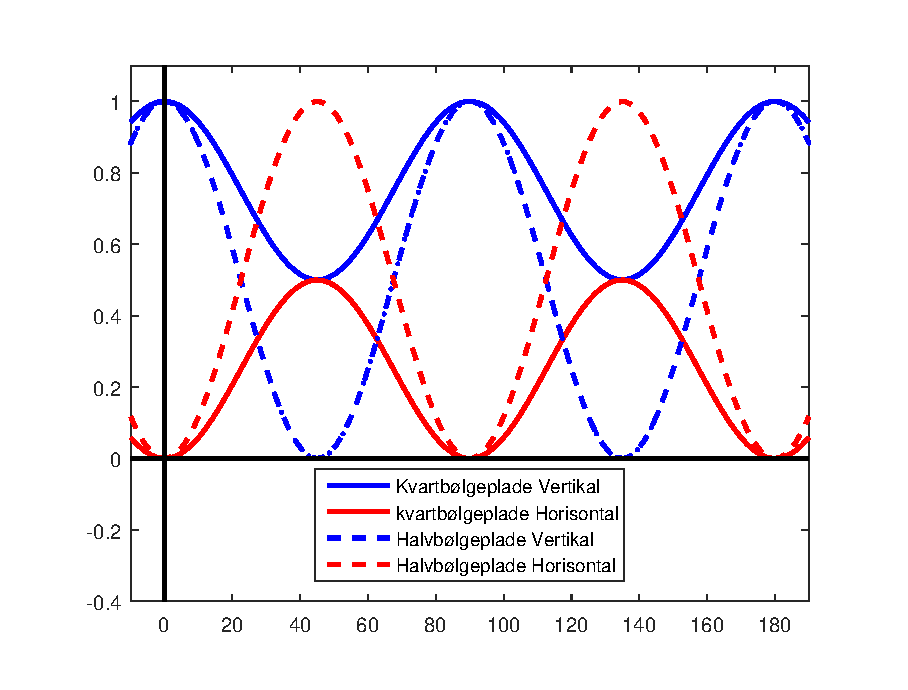
\includegraphics[width = \textwidth]{Elektrodynamik/faseskitse.eps}
\end{opgave}